\section{CmdIssuer Class Reference}
\label{classCmdIssuer}\index{CmdIssuer@{CmdIssuer}}
{\tt \#include $<$cmd\_\-issuer.h$>$}

Inheritance diagram for CmdIssuer:\nopagebreak
\begin{figure}[H]
\begin{center}
\leavevmode
\includegraphics[height=400pt]{classCmdIssuer__inherit__graph}
\end{center}
\end{figure}
Collaboration diagram for CmdIssuer:\nopagebreak
\begin{figure}[H]
\begin{center}
\leavevmode
\includegraphics[width=400pt]{classCmdIssuer__coll__graph}
\end{center}
\end{figure}
\subsection*{Public Member Functions}
\begin{CompactItemize}
\item 
{\bf CmdIssuer} ()
\item 
{\bf $\sim$CmdIssuer} ()
\item 
void {\bf process\_\-event} ({\bf IrisEvent} $\ast$e)
\item 
bool {\bf HasWork} ()
\item 
std::string {\bf toString} ()
\item 
bool {\bf IssueCmd} (bool $\ast$isWrite, {\bf DRAMCmdState} $\ast$scheduledCmd)
\item 
bool {\bf BankNotBusy} ({\bf DRAMCmdState} currentCmd)
\item 
bool {\bf BanksFirstReq} ({\bf DRAMCmdState} currentCmd, unsigned int index)
\item 
bool {\bf BusNotBusy} ({\bf DRAMCmdState} currentCmd)
\item 
bool {\bf CanSchedule} ({\bf DRAMCmdState} currentCmd, {\bf DRAMCmdState} prevCmd)
\item 
void {\bf SetBusBusyTime} ({\bf DRAMCmdState} currentCmd)
\item 
{\bf Time} {\bf CmdDelay} ({\bf DRAMCmd} cmd)
\item 
{\bf Time} {\bf CalculateDataDelay} ({\bf DRAMCmdState} cmdS)
\item 
{\bf Time} {\bf CalculateBurstL} ({\bf DRAMCmdState} prevCmd)
\item 
{\bf Time} {\bf CalculateBusyTime} ({\bf DRAMCmd} curCmd, {\bf DRAMCmd} prevCmd, {\bf RankBankComb} rankC, {\bf RankBankComb} bankC, {\bf Time} prevBurstL)
\item 
void {\bf SetPrevState} ({\bf DRAMCmdState} currentCmd)
\item 
{\bf Time} {\bf Max} ({\bf Time} t1, {\bf Time} t2)
\end{CompactItemize}
\subsection*{Public Attributes}
\begin{CompactItemize}
\item 
{\bf Component} $\ast$ {\bf parent}
\item 
{\bf DataBusHandler} $\ast$ {\bf dataBus}
\item 
{\bf CmdBusHandler} $\ast$ {\bf cmdBus}
\item 
short {\bf Id}
\item 
short {\bf bufferId}
\item 
{\bf ChannelState} {\bf prevState}
\item 
{\bf Time} {\bf busBusy}
\item 
bool {\bf generated\_\-start\_\-event}
\item 
{\bf DRAMCmd} {\bf prevBusCmd}
\end{CompactItemize}


\subsection{Detailed Description}


Definition at line 114 of file cmd\_\-issuer.h.

\subsection{Constructor \& Destructor Documentation}
\index{CmdIssuer@{CmdIssuer}!CmdIssuer@{CmdIssuer}}
\index{CmdIssuer@{CmdIssuer}!CmdIssuer@{CmdIssuer}}
\subsubsection[{CmdIssuer}]{\setlength{\rightskip}{0pt plus 5cm}CmdIssuer::CmdIssuer ()}\label{classCmdIssuer_4b8fa3fc7c33a7036f8db5c5c59a24a0}




Definition at line 27 of file cmd\_\-issuer.cc.

References busBusy, ChannelState::cmd, generated\_\-start\_\-event, NO\_\-OF\_\-BANKS, NO\_\-OF\_\-RANKS, NORMAL, PRECHARGE, ChannelState::prevCmdBank, ChannelState::prevCmdRank, ChannelState::prevCmdTime, prevState, and DRAMCmdState::set().\index{CmdIssuer@{CmdIssuer}!$\sim$CmdIssuer@{$\sim$CmdIssuer}}
\index{$\sim$CmdIssuer@{$\sim$CmdIssuer}!CmdIssuer@{CmdIssuer}}
\subsubsection[{$\sim$CmdIssuer}]{\setlength{\rightskip}{0pt plus 5cm}CmdIssuer::$\sim$CmdIssuer ()}\label{classCmdIssuer_d1406113645d9e495d9d0220539bdb77}




Definition at line 46 of file cmd\_\-issuer.cc.

\subsection{Member Function Documentation}
\index{CmdIssuer@{CmdIssuer}!BankNotBusy@{BankNotBusy}}
\index{BankNotBusy@{BankNotBusy}!CmdIssuer@{CmdIssuer}}
\subsubsection[{BankNotBusy}]{\setlength{\rightskip}{0pt plus 5cm}bool CmdIssuer::BankNotBusy ({\bf DRAMCmdState} {\em currentCmd})}\label{classCmdIssuer_5e446a025168cc448e4ad4ed70868b02}




Definition at line 244 of file cmd\_\-issuer.cc.

References ALL\_\-BANK\_\-REFRESH, Request::bankNo, CalculateBurstL(), CalculateBusyTime(), ChannelState::cmd, DRAMCmdState::cmd, NO\_\-OF\_\-BANKS, Simulator::Now(), prevState, ChannelState::rank, Request::rankNo, DRAMCmdState::req, and SAME.

Referenced by IssueCmd().

Here is the caller graph for this function:\nopagebreak
\begin{figure}[H]
\begin{center}
\leavevmode
\includegraphics[width=420pt]{classCmdIssuer_5e446a025168cc448e4ad4ed70868b02_icgraph}
\end{center}
\end{figure}
\index{CmdIssuer@{CmdIssuer}!BanksFirstReq@{BanksFirstReq}}
\index{BanksFirstReq@{BanksFirstReq}!CmdIssuer@{CmdIssuer}}
\subsubsection[{BanksFirstReq}]{\setlength{\rightskip}{0pt plus 5cm}bool CmdIssuer::BanksFirstReq ({\bf DRAMCmdState} {\em currentCmd}, \/  unsigned int {\em index})}\label{classCmdIssuer_9be81ccce536ec245fc32d5a1d661e15}




Definition at line 233 of file cmd\_\-issuer.cc.

References Request::bankNo, bufferId, BusHandler::cmdQueue, parent, and DRAMCmdState::req.

Referenced by IssueCmd().

Here is the caller graph for this function:\nopagebreak
\begin{figure}[H]
\begin{center}
\leavevmode
\includegraphics[width=420pt]{classCmdIssuer_9be81ccce536ec245fc32d5a1d661e15_icgraph}
\end{center}
\end{figure}
\index{CmdIssuer@{CmdIssuer}!BusNotBusy@{BusNotBusy}}
\index{BusNotBusy@{BusNotBusy}!CmdIssuer@{CmdIssuer}}
\subsubsection[{BusNotBusy}]{\setlength{\rightskip}{0pt plus 5cm}bool CmdIssuer::BusNotBusy ({\bf DRAMCmdState} {\em currentCmd})}\label{classCmdIssuer_f3f2fde9bf4fd88b565f372869b724d1}




Definition at line 197 of file cmd\_\-issuer.cc.

References busBusy, DRAMCmdState::cmd, Simulator::Now(), prevBusCmd, READ, t\_\-CMD, and WRITE.

Referenced by IssueCmd().

Here is the caller graph for this function:\nopagebreak
\begin{figure}[H]
\begin{center}
\leavevmode
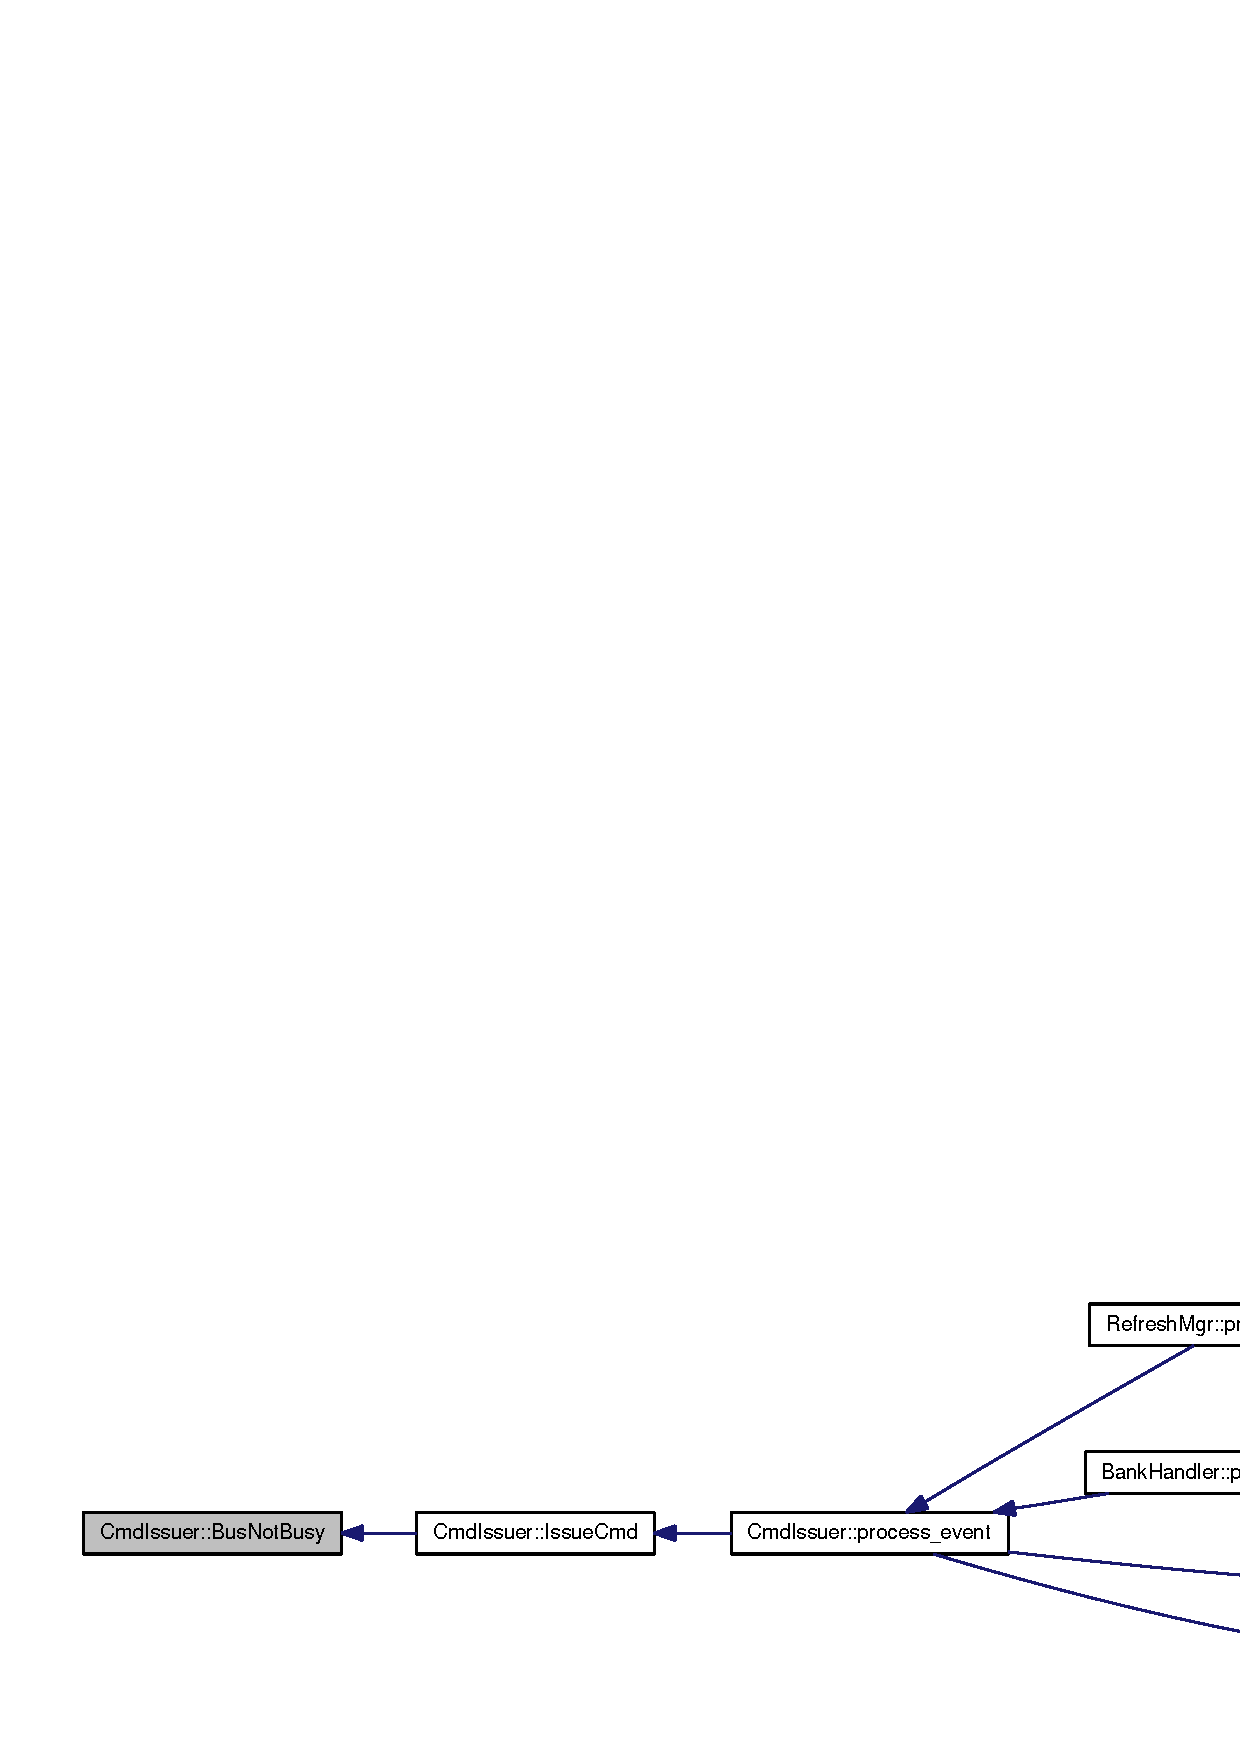
\includegraphics[width=420pt]{classCmdIssuer_f3f2fde9bf4fd88b565f372869b724d1_icgraph}
\end{center}
\end{figure}
\index{CmdIssuer@{CmdIssuer}!CalculateBurstL@{CalculateBurstL}}
\index{CalculateBurstL@{CalculateBurstL}!CmdIssuer@{CmdIssuer}}
\subsubsection[{CalculateBurstL}]{\setlength{\rightskip}{0pt plus 5cm}{\bf Time} CmdIssuer::CalculateBurstL ({\bf DRAMCmdState} {\em prevCmd})}\label{classCmdIssuer_4f8af3e538cf545ef379e2a4da7b8a38}




Definition at line 334 of file cmd\_\-issuer.cc.

References DRAMCmdState::burst, BUS\_\-CYCLE, DDR\_\-BUS\_\-WIDTH, PREFETCH\_\-SIZE, PREFETCHL, READ\_\-SIZE, READL, WRITE\_\-SIZE, WRITEBACK\_\-SIZE, WRITEBACKL, and WRITEL.

Referenced by BankNotBusy(), CanSchedule(), and SetBusBusyTime().

Here is the caller graph for this function:\nopagebreak
\begin{figure}[H]
\begin{center}
\leavevmode
\includegraphics[width=420pt]{classCmdIssuer_4f8af3e538cf545ef379e2a4da7b8a38_icgraph}
\end{center}
\end{figure}
\index{CmdIssuer@{CmdIssuer}!CalculateBusyTime@{CalculateBusyTime}}
\index{CalculateBusyTime@{CalculateBusyTime}!CmdIssuer@{CmdIssuer}}
\subsubsection[{CalculateBusyTime}]{\setlength{\rightskip}{0pt plus 5cm}{\bf Time} CmdIssuer::CalculateBusyTime ({\bf DRAMCmd} {\em curCmd}, \/  {\bf DRAMCmd} {\em prevCmd}, \/  {\bf RankBankComb} {\em rankC}, \/  {\bf RankBankComb} {\em bankC}, \/  {\bf Time} {\em prevBurstL})}\label{classCmdIssuer_46557041a802ab092db4a9a3738ac142}




Definition at line 357 of file cmd\_\-issuer.cc.

References ACTIVATE, ALL\_\-BANK\_\-REFRESH, CLOSE\_\-PAGE\_\-POLICY, DIFF, dram\_\-page\_\-policy, Max(), OPEN\_\-PAGE\_\-POLICY, PRECHARGE, READ, SAME, t\_\-AL, t\_\-CAS, t\_\-CCD, t\_\-CMD, t\_\-CWD, t\_\-OST, t\_\-RAS, t\_\-RCD, t\_\-RFC, t\_\-RP, t\_\-RRD, t\_\-RTP, t\_\-RTRS, t\_\-WR, t\_\-WTR, and WRITE.

Referenced by BankNotBusy(), and CanSchedule().

Here is the caller graph for this function:\nopagebreak
\begin{figure}[H]
\begin{center}
\leavevmode
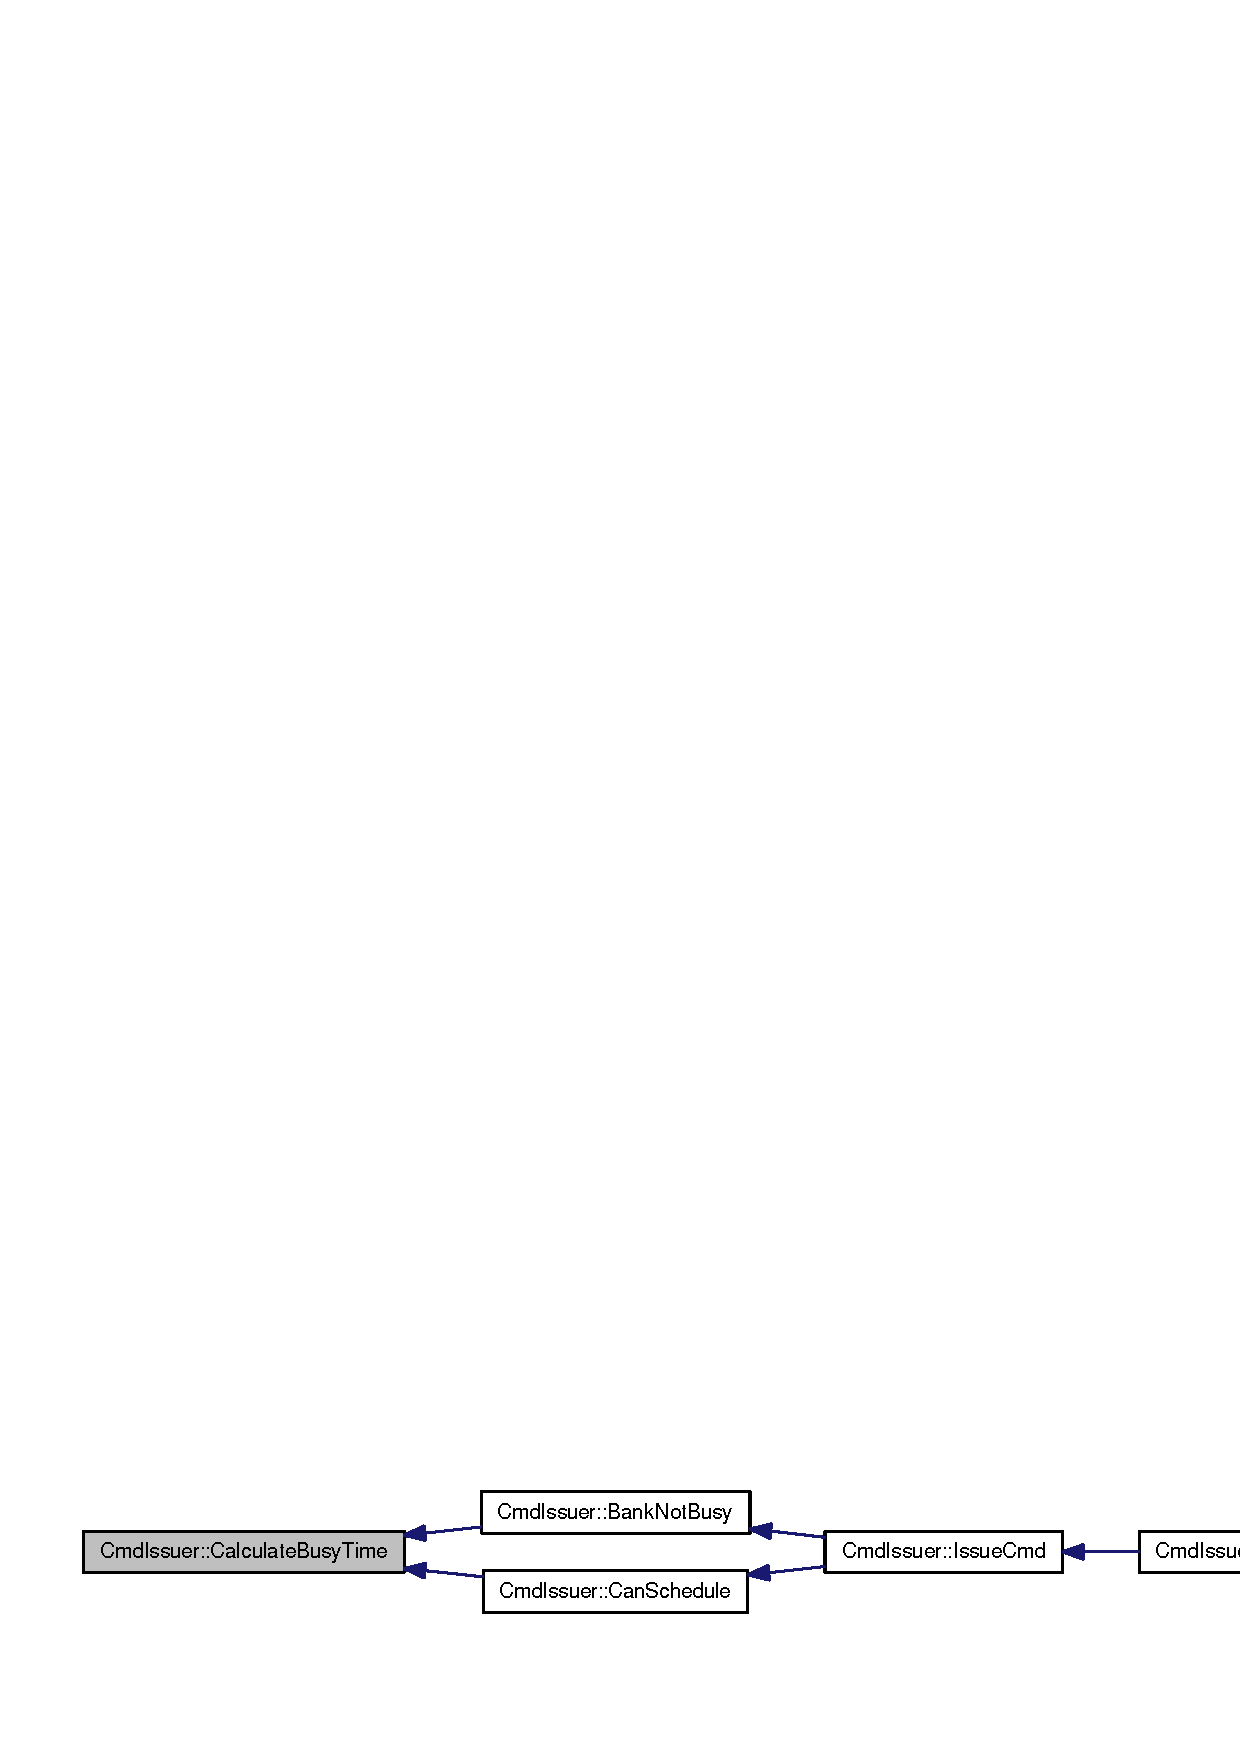
\includegraphics[width=420pt]{classCmdIssuer_46557041a802ab092db4a9a3738ac142_icgraph}
\end{center}
\end{figure}
\index{CmdIssuer@{CmdIssuer}!CalculateDataDelay@{CalculateDataDelay}}
\index{CalculateDataDelay@{CalculateDataDelay}!CmdIssuer@{CmdIssuer}}
\subsubsection[{CalculateDataDelay}]{\setlength{\rightskip}{0pt plus 5cm}{\bf Time} CmdIssuer::CalculateDataDelay ({\bf DRAMCmdState} {\em cmdS})}\label{classCmdIssuer_4455c4f070b8d8f9e6ae11a1e972b955}




Definition at line 297 of file cmd\_\-issuer.cc.

References DRAMCmdState::cmd, t\_\-CMD, t\_\-CWD, and WRITE.

Referenced by process\_\-event().

Here is the caller graph for this function:\nopagebreak
\begin{figure}[H]
\begin{center}
\leavevmode
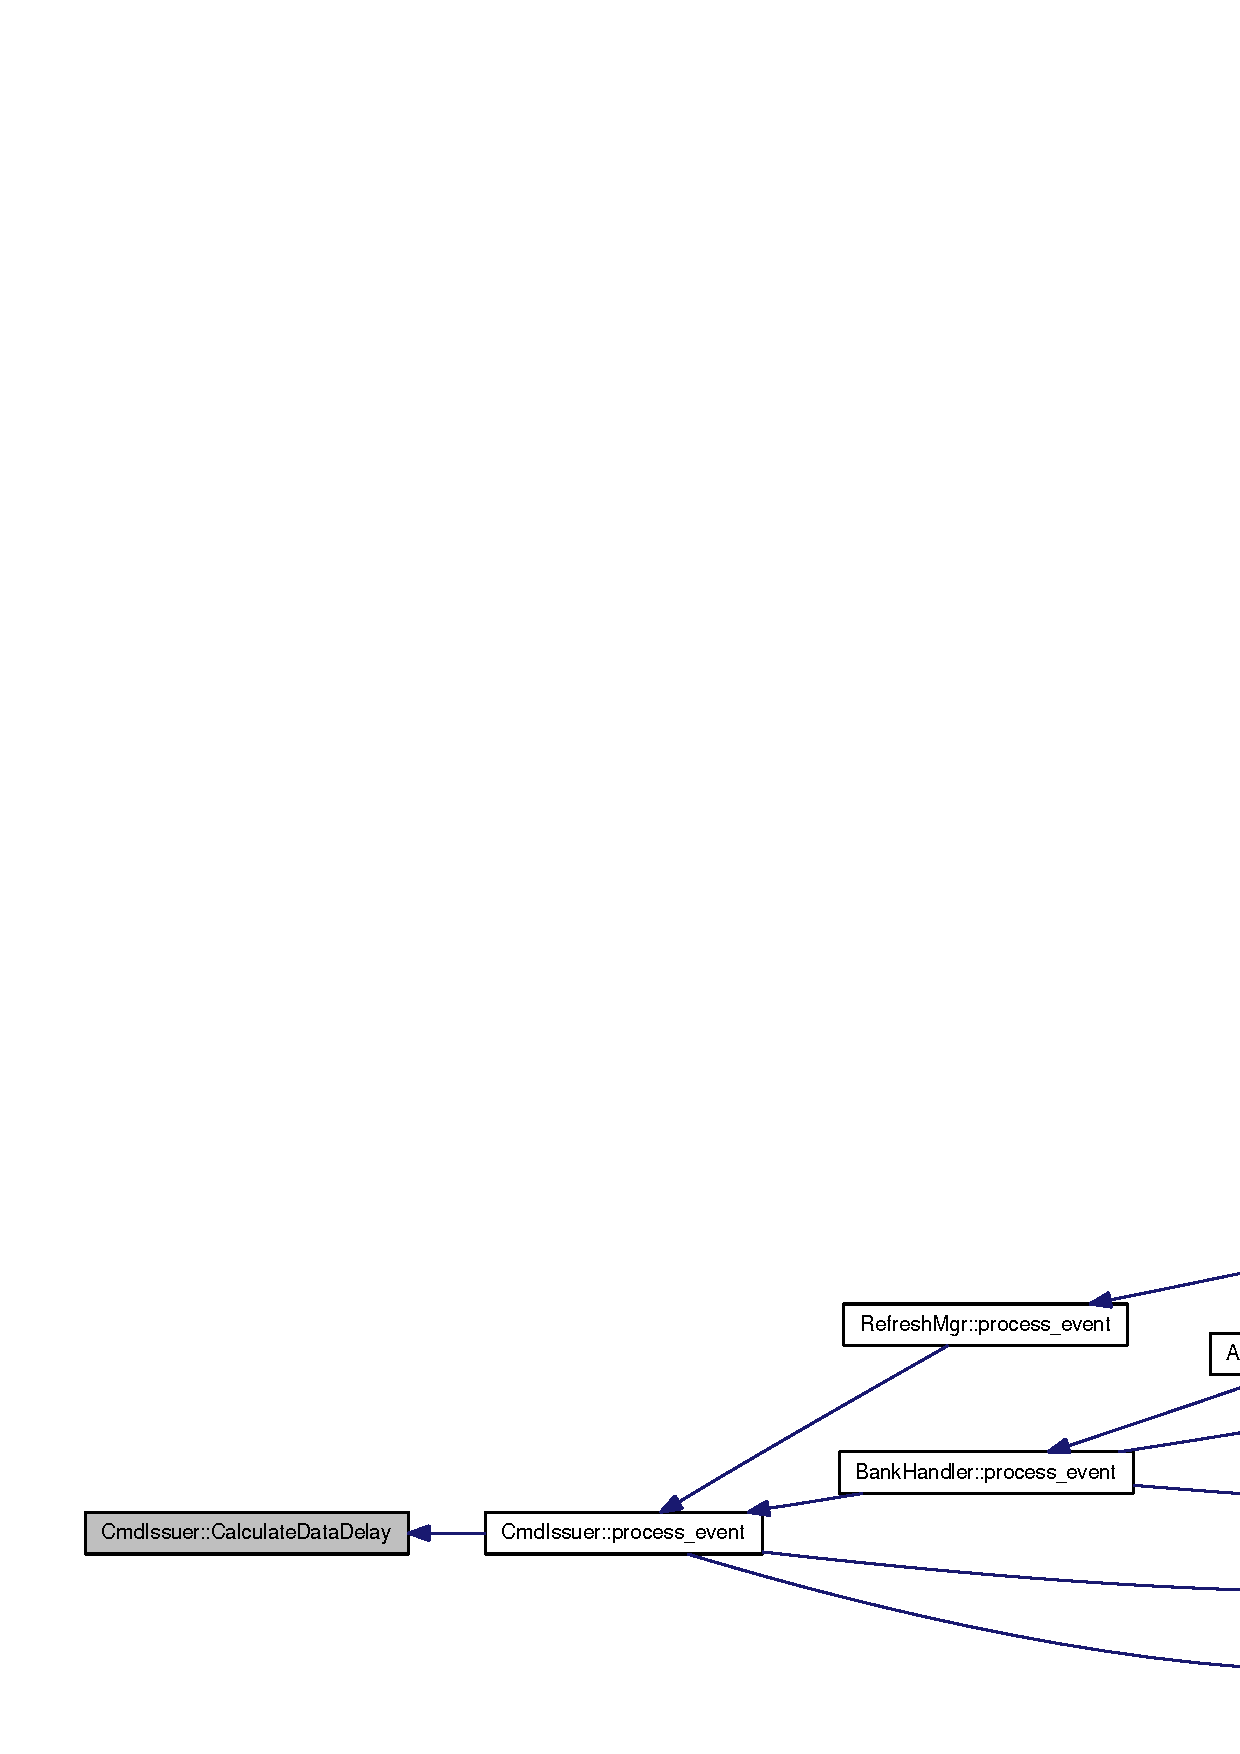
\includegraphics[width=420pt]{classCmdIssuer_4455c4f070b8d8f9e6ae11a1e972b955_icgraph}
\end{center}
\end{figure}
\index{CmdIssuer@{CmdIssuer}!CanSchedule@{CanSchedule}}
\index{CanSchedule@{CanSchedule}!CmdIssuer@{CmdIssuer}}
\subsubsection[{CanSchedule}]{\setlength{\rightskip}{0pt plus 5cm}bool CmdIssuer::CanSchedule ({\bf DRAMCmdState} {\em currentCmd}, \/  {\bf DRAMCmdState} {\em prevCmd})}\label{classCmdIssuer_4a1322edbe59ad37ce4cfe32cf42f662}




Definition at line 309 of file cmd\_\-issuer.cc.

References Request::bankNo, CalculateBurstL(), CalculateBusyTime(), DRAMCmdState::cmd, DIFF, Simulator::Now(), ChannelState::prevCmdTime, prevState, Request::rankNo, DRAMCmdState::req, and SAME.

Referenced by IssueCmd().

Here is the caller graph for this function:\nopagebreak
\begin{figure}[H]
\begin{center}
\leavevmode
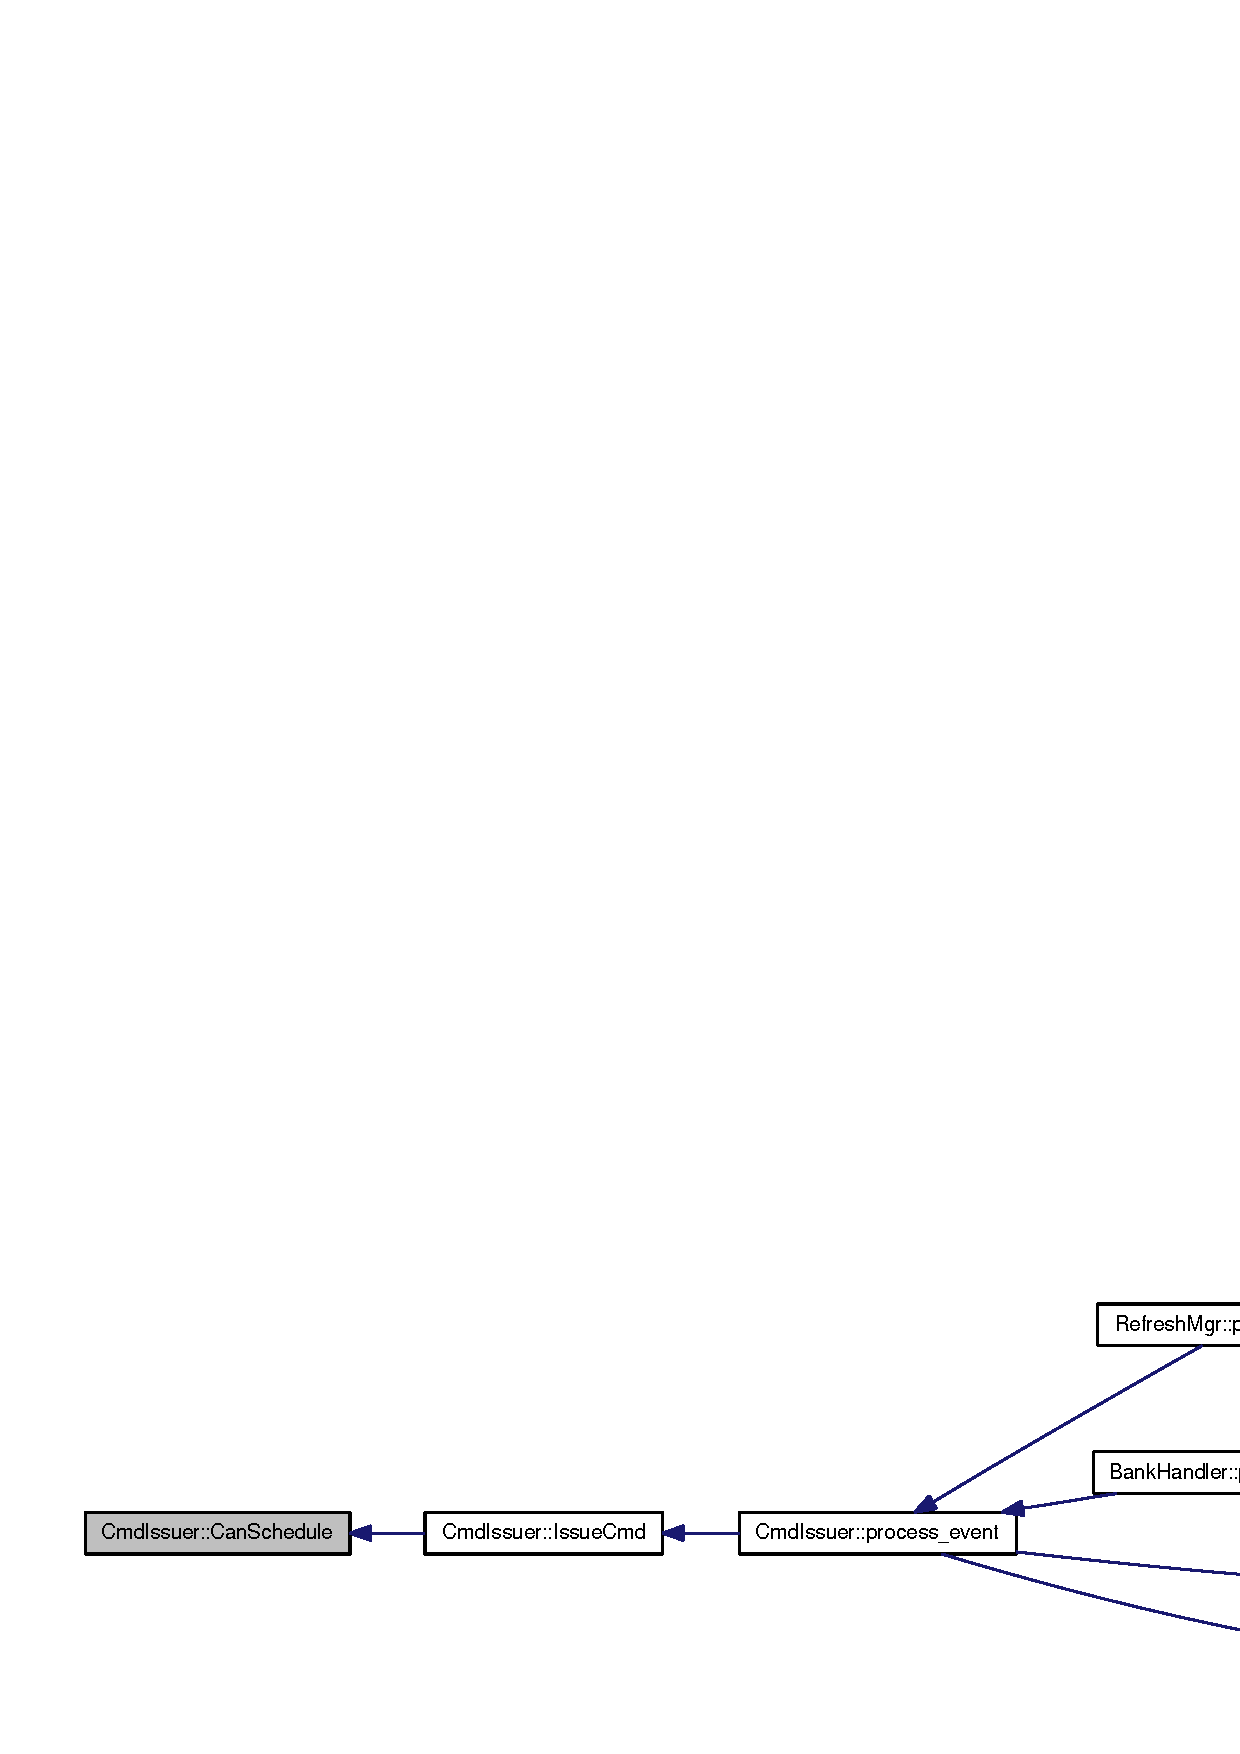
\includegraphics[width=420pt]{classCmdIssuer_4a1322edbe59ad37ce4cfe32cf42f662_icgraph}
\end{center}
\end{figure}
\index{CmdIssuer@{CmdIssuer}!CmdDelay@{CmdDelay}}
\index{CmdDelay@{CmdDelay}!CmdIssuer@{CmdIssuer}}
\subsubsection[{CmdDelay}]{\setlength{\rightskip}{0pt plus 5cm}{\bf Time} CmdIssuer::CmdDelay ({\bf DRAMCmd} {\em cmd})}\label{classCmdIssuer_a24df46861dc460b678957f7bef64631}




Definition at line 281 of file cmd\_\-issuer.cc.

References ACTIVATE, ALL\_\-BANK\_\-REFRESH, PRECHARGE, READ, t\_\-CAS, t\_\-RCD, t\_\-RFC, t\_\-RP, and WRITE.\index{CmdIssuer@{CmdIssuer}!HasWork@{HasWork}}
\index{HasWork@{HasWork}!CmdIssuer@{CmdIssuer}}
\subsubsection[{HasWork}]{\setlength{\rightskip}{0pt plus 5cm}bool CmdIssuer::HasWork ()}\label{classCmdIssuer_feb7f8dea256a6352ec8cf65ec0dd484}




Definition at line 149 of file cmd\_\-issuer.cc.

References bufferId, and parent.

Referenced by process\_\-event().

Here is the caller graph for this function:\nopagebreak
\begin{figure}[H]
\begin{center}
\leavevmode
\includegraphics[width=420pt]{classCmdIssuer_feb7f8dea256a6352ec8cf65ec0dd484_icgraph}
\end{center}
\end{figure}
\index{CmdIssuer@{CmdIssuer}!IssueCmd@{IssueCmd}}
\index{IssueCmd@{IssueCmd}!CmdIssuer@{CmdIssuer}}
\subsubsection[{IssueCmd}]{\setlength{\rightskip}{0pt plus 5cm}bool CmdIssuer::IssueCmd (bool $\ast$ {\em isWrite}, \/  {\bf DRAMCmdState} $\ast$ {\em scheduledCmd})}\label{classCmdIssuer_7bff6a1ba1f511a08925d9bd55a47cab}




Definition at line 159 of file cmd\_\-issuer.cc.

References BankNotBusy(), BanksFirstReq(), bufferId, BusNotBusy(), CanSchedule(), ChannelState::cmd, BusHandler::cmdQueue, parent, prevState, SetBusBusyTime(), SetPrevState(), and WRITE.

Referenced by process\_\-event().

Here is the caller graph for this function:\nopagebreak
\begin{figure}[H]
\begin{center}
\leavevmode
\includegraphics[width=420pt]{classCmdIssuer_7bff6a1ba1f511a08925d9bd55a47cab_icgraph}
\end{center}
\end{figure}
\index{CmdIssuer@{CmdIssuer}!Max@{Max}}
\index{Max@{Max}!CmdIssuer@{CmdIssuer}}
\subsubsection[{Max}]{\setlength{\rightskip}{0pt plus 5cm}{\bf Time} CmdIssuer::Max ({\bf Time} {\em t1}, \/  {\bf Time} {\em t2})}\label{classCmdIssuer_2737bf8ac4ff1dd206404866fa8666e6}




Definition at line 731 of file cmd\_\-issuer.cc.

Referenced by CalculateBusyTime().

Here is the caller graph for this function:\nopagebreak
\begin{figure}[H]
\begin{center}
\leavevmode
\includegraphics[width=420pt]{classCmdIssuer_2737bf8ac4ff1dd206404866fa8666e6_icgraph}
\end{center}
\end{figure}
\index{CmdIssuer@{CmdIssuer}!process\_\-event@{process\_\-event}}
\index{process\_\-event@{process\_\-event}!CmdIssuer@{CmdIssuer}}
\subsubsection[{process\_\-event}]{\setlength{\rightskip}{0pt plus 5cm}void CmdIssuer::process\_\-event ({\bf IrisEvent} $\ast$ {\em e})}\label{classCmdIssuer_37cfadf3b2fe7118c26dc5bdee0e92b0}




Definition at line 58 of file cmd\_\-issuer.cc.

References Request::address, Request::bankNo, Request::busInsertionTime, CalculateDataDelay(), Request::channelNo, CLOSE\_\-PAGE\_\-POLICY, DRAMCmdState::cmd, cmdBus, dataBus, dram\_\-page\_\-policy, IrisEvent::dst, IrisEvent::event\_\-data, generated\_\-start\_\-event, HasWork(), Id, IssueCmd(), Simulator::Now(), OPEN\_\-PAGE\_\-POLICY, parent, PRECHARGE, DataBusHandler::process\_\-event(), CmdBusHandler::process\_\-event(), Request::rankNo, READ, DRAMCmdState::req, Simulator::Schedule(), IrisEvent::src, START, START\_\-WRITE, IrisEvent::type, and WRITE.

Referenced by RefreshMgr::process\_\-event(), and BankHandler::process\_\-event().

Here is the caller graph for this function:\nopagebreak
\begin{figure}[H]
\begin{center}
\leavevmode
\includegraphics[width=420pt]{classCmdIssuer_37cfadf3b2fe7118c26dc5bdee0e92b0_icgraph}
\end{center}
\end{figure}
\index{CmdIssuer@{CmdIssuer}!SetBusBusyTime@{SetBusBusyTime}}
\index{SetBusBusyTime@{SetBusBusyTime}!CmdIssuer@{CmdIssuer}}
\subsubsection[{SetBusBusyTime}]{\setlength{\rightskip}{0pt plus 5cm}void CmdIssuer::SetBusBusyTime ({\bf DRAMCmdState} {\em currentCmd})}\label{classCmdIssuer_cad3d934f37eeea768b3eca35b56b558}




Definition at line 220 of file cmd\_\-issuer.cc.

References busBusy, CalculateBurstL(), DRAMCmdState::cmd, Simulator::Now(), prevBusCmd, READ, and WRITE.

Referenced by IssueCmd().

Here is the caller graph for this function:\nopagebreak
\begin{figure}[H]
\begin{center}
\leavevmode
\includegraphics[width=420pt]{classCmdIssuer_cad3d934f37eeea768b3eca35b56b558_icgraph}
\end{center}
\end{figure}
\index{CmdIssuer@{CmdIssuer}!SetPrevState@{SetPrevState}}
\index{SetPrevState@{SetPrevState}!CmdIssuer@{CmdIssuer}}
\subsubsection[{SetPrevState}]{\setlength{\rightskip}{0pt plus 5cm}void CmdIssuer::SetPrevState ({\bf DRAMCmdState} {\em currentCmd})}\label{classCmdIssuer_bd3ac25d8c718c66445a2e92bb97df0e}




Definition at line 719 of file cmd\_\-issuer.cc.

References Request::bankNo, DRAMCmdState::cmd, ChannelState::cmd, Simulator::Now(), ChannelState::prevCmdBank, ChannelState::prevCmdRank, ChannelState::prevCmdTime, prevState, ChannelState::rank, Request::rankNo, DRAMCmdState::req, and Request::rowNo.

Referenced by IssueCmd().

Here is the caller graph for this function:\nopagebreak
\begin{figure}[H]
\begin{center}
\leavevmode
\includegraphics[width=420pt]{classCmdIssuer_bd3ac25d8c718c66445a2e92bb97df0e_icgraph}
\end{center}
\end{figure}
\index{CmdIssuer@{CmdIssuer}!toString@{toString}}
\index{toString@{toString}!CmdIssuer@{CmdIssuer}}
\subsubsection[{toString}]{\setlength{\rightskip}{0pt plus 5cm}std::string CmdIssuer::toString ()}\label{classCmdIssuer_0f974d7bee65d627f6247f2b970cf1d9}




Definition at line 154 of file cmd\_\-issuer.cc.

\subsection{Member Data Documentation}
\index{CmdIssuer@{CmdIssuer}!bufferId@{bufferId}}
\index{bufferId@{bufferId}!CmdIssuer@{CmdIssuer}}
\subsubsection[{bufferId}]{\setlength{\rightskip}{0pt plus 5cm}short {\bf CmdIssuer::bufferId}}\label{classCmdIssuer_5349d862a11425e1feeb656149341352}




Definition at line 123 of file cmd\_\-issuer.h.

Referenced by BanksFirstReq(), BusHandler::BusHandler(), HasWork(), and IssueCmd().\index{CmdIssuer@{CmdIssuer}!busBusy@{busBusy}}
\index{busBusy@{busBusy}!CmdIssuer@{CmdIssuer}}
\subsubsection[{busBusy}]{\setlength{\rightskip}{0pt plus 5cm}{\bf Time} {\bf CmdIssuer::busBusy}}\label{classCmdIssuer_a39f3a34916eca57871a8d44820c50a8}




Definition at line 125 of file cmd\_\-issuer.h.

Referenced by BusNotBusy(), CmdIssuer(), and SetBusBusyTime().\index{CmdIssuer@{CmdIssuer}!cmdBus@{cmdBus}}
\index{cmdBus@{cmdBus}!CmdIssuer@{CmdIssuer}}
\subsubsection[{cmdBus}]{\setlength{\rightskip}{0pt plus 5cm}{\bf CmdBusHandler}$\ast$ {\bf CmdIssuer::cmdBus}}\label{classCmdIssuer_51c081738a59757304b5cb1955a4b016}




Definition at line 121 of file cmd\_\-issuer.h.

Referenced by process\_\-event(), and RequestHandler::SetLinks().\index{CmdIssuer@{CmdIssuer}!dataBus@{dataBus}}
\index{dataBus@{dataBus}!CmdIssuer@{CmdIssuer}}
\subsubsection[{dataBus}]{\setlength{\rightskip}{0pt plus 5cm}{\bf DataBusHandler}$\ast$ {\bf CmdIssuer::dataBus}}\label{classCmdIssuer_6f0d862a1a30aa215a5df5df54ffb274}




Definition at line 120 of file cmd\_\-issuer.h.

Referenced by process\_\-event(), and RequestHandler::SetLinks().\index{CmdIssuer@{CmdIssuer}!generated\_\-start\_\-event@{generated\_\-start\_\-event}}
\index{generated\_\-start\_\-event@{generated\_\-start\_\-event}!CmdIssuer@{CmdIssuer}}
\subsubsection[{generated\_\-start\_\-event}]{\setlength{\rightskip}{0pt plus 5cm}bool {\bf CmdIssuer::generated\_\-start\_\-event}}\label{classCmdIssuer_e2dca7df5ab6300cd97bb7b90af25d25}




Definition at line 142 of file cmd\_\-issuer.h.

Referenced by CmdIssuer(), and process\_\-event().\index{CmdIssuer@{CmdIssuer}!Id@{Id}}
\index{Id@{Id}!CmdIssuer@{CmdIssuer}}
\subsubsection[{Id}]{\setlength{\rightskip}{0pt plus 5cm}short {\bf CmdIssuer::Id}}\label{classCmdIssuer_cac87f00286cca7f0a03dce0542f6fde}




Definition at line 122 of file cmd\_\-issuer.h.

Referenced by BusHandler::BusHandler(), and process\_\-event().\index{CmdIssuer@{CmdIssuer}!parent@{parent}}
\index{parent@{parent}!CmdIssuer@{CmdIssuer}}
\subsubsection[{parent}]{\setlength{\rightskip}{0pt plus 5cm}{\bf Component}$\ast$ {\bf CmdIssuer::parent}}\label{classCmdIssuer_5e1ed2ce5508ea4bd898bbc6f46fd8ba}




Definition at line 119 of file cmd\_\-issuer.h.

Referenced by BanksFirstReq(), BusHandler::BusHandler(), HasWork(), IssueCmd(), and process\_\-event().\index{CmdIssuer@{CmdIssuer}!prevBusCmd@{prevBusCmd}}
\index{prevBusCmd@{prevBusCmd}!CmdIssuer@{CmdIssuer}}
\subsubsection[{prevBusCmd}]{\setlength{\rightskip}{0pt plus 5cm}{\bf DRAMCmd} {\bf CmdIssuer::prevBusCmd}}\label{classCmdIssuer_83305626c36c8db41d32b0c30dce8fff}




Definition at line 143 of file cmd\_\-issuer.h.

Referenced by BusNotBusy(), and SetBusBusyTime().\index{CmdIssuer@{CmdIssuer}!prevState@{prevState}}
\index{prevState@{prevState}!CmdIssuer@{CmdIssuer}}
\subsubsection[{prevState}]{\setlength{\rightskip}{0pt plus 5cm}{\bf ChannelState} {\bf CmdIssuer::prevState}}\label{classCmdIssuer_cde77c9f037d0c964a05355d3afeeb1a}




Definition at line 124 of file cmd\_\-issuer.h.

Referenced by BankNotBusy(), CanSchedule(), CmdIssuer(), IssueCmd(), and SetPrevState().

The documentation for this class was generated from the following files:\begin{CompactItemize}
\item 
{\bf cmd\_\-issuer.h}\item 
{\bf cmd\_\-issuer.cc}\end{CompactItemize}
